\section{Analysis \& Methods}	\label{sec:analysis-methods}
Due to the inherent characteristics of the VOIP (Voice over IP) application, a series of protocols and mechanisms have been designed to ensure the quality of VoIP communication. One task of the experiments is protocol research, including analyzing the collaboration between the protocols included in the process and finding out the principles of the VoIP application design.

According to the "branch exchange" scheme, the first step is building the link, of which the responsibility is taken by the Session Initiation Protocol (SIP).


\subsection{Basic SIP Analysis}
The Session Initiation Protocol (SIP) is an application layer control protocol for establishing, changing and terminating multimedia sessions, where the sessions can be IP telephony, multimedia sessions or multimedia conferences. SIP is the core protocol of many IP-based PBX applications, including Asterisk.

\begin{figure}[htbp]
	\centerline{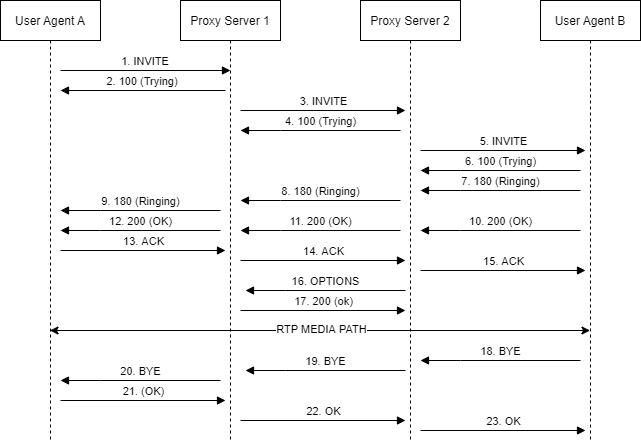
\includegraphics[width=8cm]{Images/experiment/SIP.png}}
	\caption{Session Initialization in SIP model}
	\label{fig:sip}
\end{figure}



As shown in Fig.\ref{fig:sip}, the SIP process starts with registration. All SIP terminals as User Agents should register with the registration server to inform their location, session capability, and other information.

Usually, when the SIP terminal (User Agent) is powered on or configured to perform a registration operation, a registration request message (REGISTER) is sent to the registration server, carrying all the information that needs to be registered. After receiving the registration request message, the registration server sends a response message to the terminal to inform it that the request message has been received. If the registration is successful, it will send a "200 OK" message to the terminal. However, the most common response is a "401 Unauthorized" message because authorization is required in most of the implementations for security purposes. 

The SIP protocol adopts the Client-Server pattern, in which the calls are established between User Agents through the proxy server.

Upon the link built by SIP, the data transmission tasks are carried out with RTP/RTCP protocol.

\subsection{RTP}
RTP is a real-time protocol for transmitting audio and video streams over IP networks. For telephony applications, the data consists of voice spurts, instead of being a stable data flow. So each RTP packet only contains a small sample of voice messages, whose length is usually 20 to 30 ms.

RTP introduces two fields into its header, the sequence number and the timestamp, generated by the sender devices.

\subsection{RTCP}
RTCP is a control protocol accompanied by RTP, providing the report of the RTP stream received by the destination devices. So RTCP packets always head in the reverse direction of RTP streams. After checking the RTCP report, the sender updates the transmission strategy to adapt to the network condition.

\subsection{Jitter and Packet loss}
VoIP applications are sensitive to jitter. In VoIP calls, the voice stream consists of alternating talk spurts and silent periods. Since silent periods separate the discrete valuable voice messages, the timing and the sequence of the packets' arrival are very important. Voice packets that are out of order may not be decoded correctly. Jitter has a large impact on the sequence of the arriving RTP packets. If the packets arrive at even intervals in the correct order, the jitter is low. Reversely, if the packets arrive in bursts or out of order, the jitter is high.

Compared with jitter, packet loss can be tolerant because it does not change the sequence and time of the packet. So the packet loss that is under a threshold, usually under 3\% can be accepted.

In the experiment, jitter has been applied as an important indicator to evaluate the quality of the VoIP calls.


\subsection{Basic Network Topology}
To demonstrate the main components of the SIP communication, a simplified scenario is implemented, as shown in Figure  \hyperref[fig:topo]{Figure \ref{fig:topo}}. Two VoIP applications are running on the same computer, and an IP-based PBX application (Asterisk), running on a Raspberry Pi 4, is serving as the PBX server.

\begin{figure}[htbp]
	\centerline{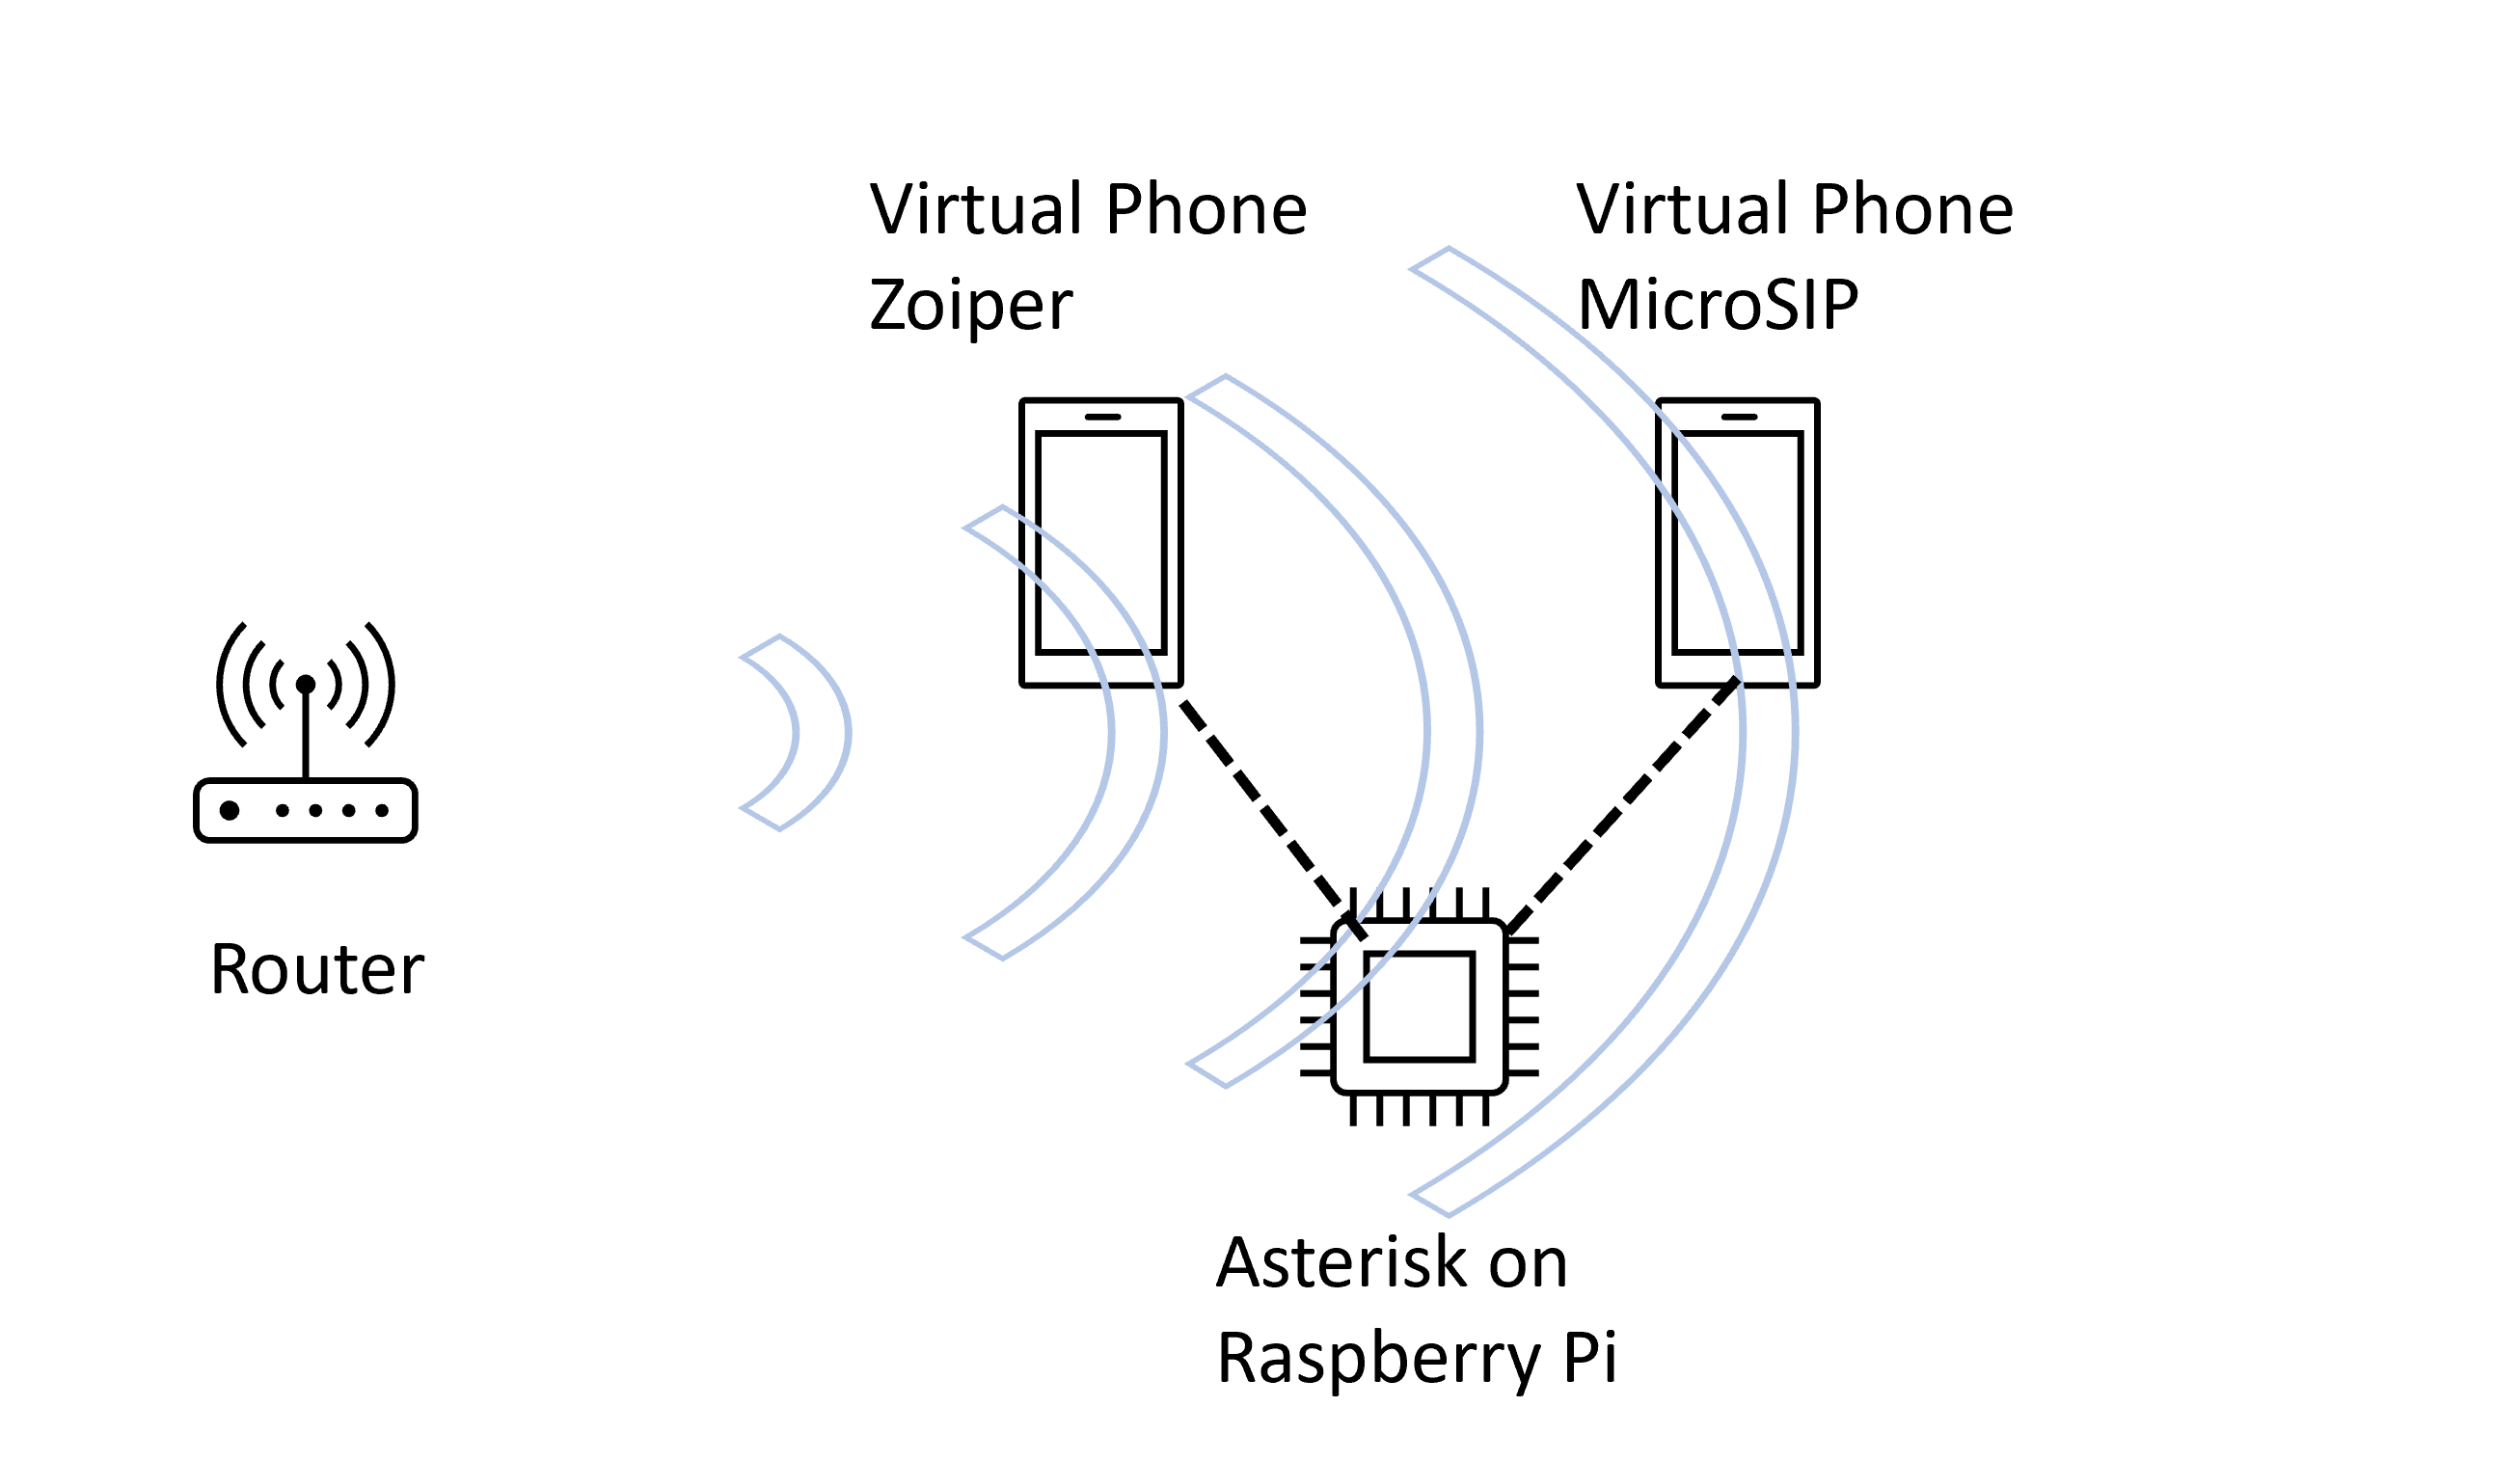
\includegraphics[width=8cm]{Images/experiment/exp1.png}}
	\caption{Simplified Scenario}
	\label{fig:topo}
\end{figure}

To trace and see all types of packets transmissions, author used Wireshark open-source software. \hyperref[fig:packet-trace]{Figure \ref{fig:packet-trace}} is a flow sequence of the one single call from Zoiper5 user (IP: 192.168.60.106:63771) to MicroSIP user (IP:192.168.60.106:53493). In this, scenario their are actual two connections, first from Zoiper5 user to Asterisk (shown in left-side of Figure \ref{fig:packet-trace}) and second Asterisk to MicroSIP (shown in right-side of Figure \ref{fig:packet-trace}).

\begin{figure}[htbp]
	\begin{minipage}{0.24\textwidth}
		\begin{flushleft}
			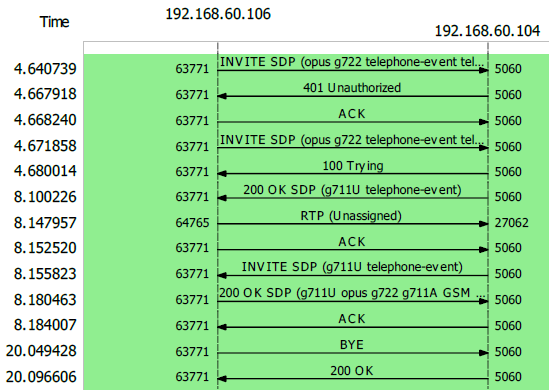
\includegraphics[height=100pt,width=\textwidth]{Images/experiment/a1.png}
			%%					\caption{Zoiper to Asterisk}
		\end{flushleft}
	\end{minipage}
	\begin{minipage}{0.24\textwidth}
		\begin{flushright}
			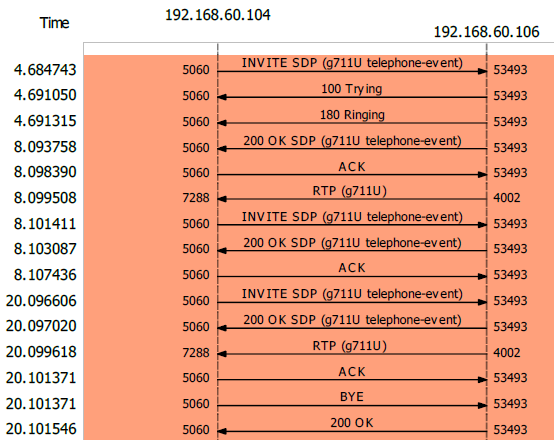
\includegraphics[height=100pt,width=\textwidth]{Images/experiment/a2.png}
			%					\caption{Zoiper to MicroSIP}
		\end{flushright}
	\end{minipage}
	\caption{SIP packet transmission from Zoiper to Asterisk(left-side), Asterisk to MicroSIP (right-side)}
	\label{fig:packet-trace}
\end{figure}